\section[Общесистемная часть]{ОБЩЕСИСТЕМНАЯ ЧАСТЬ}

\subsection{Описание объекта проектирования}

Объектом проектирования является мобильное приложение,
отображающее актуальную информацию о курсах валют
в Республике Беларусь.

Ввод данных осуществляется в автоматическом режиме,
используя API сайта myfin.by. В качестве параметра запроса
используется индекс областного центра Республики Беларусь.

Хранение данных осуществляется средствами мобильной бызы данных Realm~\cite{realm}.

Вывод данных сводится к отображению актуальных курсов валют в виде списка,
максимальных и минимальных значений стоимостей валют,
а также детальное отображение информации об отделении.


\subsection{Постановка задачи проектирования}

Требуется выполнить проектирование автоматизированной системы,
выполненной в виде мобильного приложения и обладающей следующими
функциональными возможностями:
\begin{itemize}
  \item автоматический ввод данных о курсах валют в зависимости
    от местоположения пользователя;  
  \item использование приложения без доступа к интернету;
  \item приоритетное отображение информации о выбранных пользователем отделениях; 
  \item наглядное отображение местоположения конкретного отделения;
  \item группировка данных по валютам;
  \item отображение максимальных, средних значений курсов;
  \item сравнение курсов валют в коммерческих банках
    с курсом Национального банка Республики Беларусь;
  \item использование конвертера валют.
\end{itemize}

Разработанное приложение должно соответствовать документу,
содержащему рекомендации по разработке программного обеспечения для
iOS устройств, разработанному компанией Apple~\cite{ios_hig}.

Оформление работы требуется выполнить в соответствии
со стандартом оформления курсовых и дипломных работ~\cite{stp2013}.


\pagebreak
\subsection{Концептуальная модель системы}

Можно выделить следующие сценарии использования приложения:
\begin{itemize}
  \item просмотр курсов валют;
  \item использование конвертер валют;
  \item выполнение поиска по отделениям;
  \item изменение пользовательских настроек;
\end{itemize}

Эти сценарии приведены на рисунке~\ref{fig:use_case}.

\begin{figure}[h!]
  \centering
  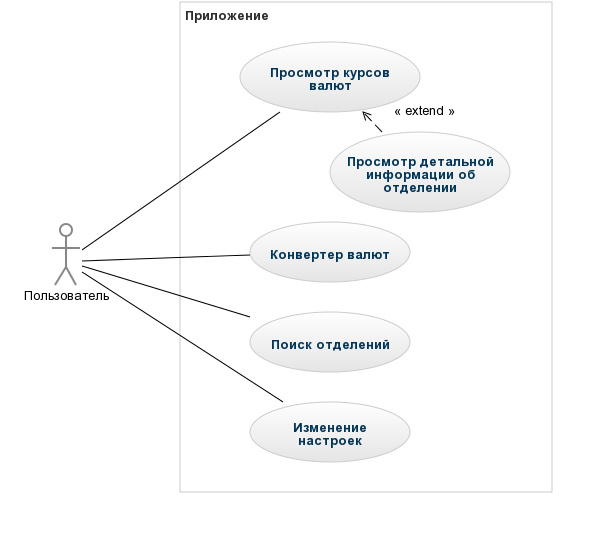
\includegraphics[width=140mm]{pic/use_case}
  \caption{Диаграмма прецендентов \\ использования приложения}
  \label{fig:use_case}
\end{figure}

Ввод финансовых данных предполагается совершать в автоматическом режиме
с учётом выбранного пользователем местоположения.
Просмотр информации о курсах предполагает выборку требуемой информации
из базы данных и её представление в наглядной форме. 

Можно выделить следующие сущности рассматриваемой
предметной области:
\begin{itemize}
  \item банки;
  \item отделения;
  \item курсы.
\end{itemize}

Эти сущности, а также связи между ними, приведены на рисунке~\ref{fig:entities}.

Сущность <<Банк>> соответствует общей информации о банке
и состоит из идентификатора, названия и сайта банка.

Сущность <<Отделение>> соответствует информации об отделении банка
и состоит из идентификатора, названия, адреса, телефона, координат.

Сущность <<Курс>> содержит данные о курсах валют.

\begin{figure}[h!]
  \centering
  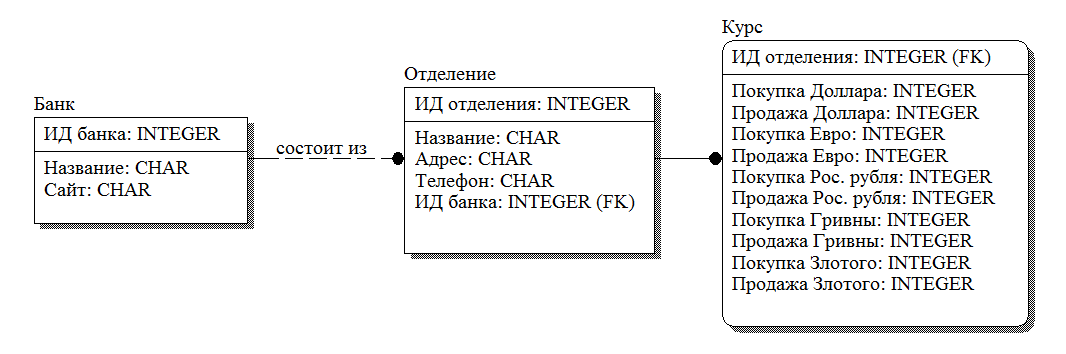
\includegraphics[width=150mm]{pic/entities}
  \caption{Основные сущности \\ предметной области}
  \label{fig:entities}
\end{figure}

Сущности <<Банк>> и <<Отделение>> связаны связью
вида один-ко-многим, так как одному банку может соответствовать
множество его дочерних отделений.

Сущность <<Отделение>> и <<Курс>> связаны связью один-к-одному,
так как каждому отделению соответствуют только один набор курсов валют.
